\documentclass[a4paper,11pt]{article}
\usepackage[utf8]{inputenc}
\usepackage[english]{babel}
\usepackage{graphicx}
\usepackage{subcaption}
\usepackage{chngcntr}
\counterwithin{figure}{section}
\usepackage{authblk}
\usepackage{titling}
\setlength{\droptitle}{-5em}   % This eliminates the space on top of title
\usepackage[font=scriptsize]{caption}
\usepackage{float}
\usepackage{siunitx}
\usepackage{hyperref}
\usepackage{geometry}
\geometry{legalpaper, margin=1in}

\usepackage{biblatex}

\addbibresource{references.bib}

%opening
\title{DisCease\\A Complex Systems And Networks Project}
\author{Akhil Devarashetti, Jenna Sawaf}

\begin{document}
    \maketitle

    \begin{abstract}
        We tried to create a model that simulates the spread of a disease that does not have a medicine.
        We observed the effects of varying parameters, then introduced a concept of deflections which mimic social distancing and social gatherings.
        We finally made an attempt to evolve these deflections based on a performance metric.
    \end{abstract}

    \section{Introduction}\label{sec:introduction}
    During February 2020, the outbreak of COVID-19 was starting to become a pandemic.
    We recognized that this percolation is a complex systems problem.
    We started this project with the goal of developing a model that simulates COVID-19-like epidemics and study the behaviour of the agents in order to determine the best behaviours to mitigate the spread of the disease, hence, the name DisCease.

    We created a modified SIR model\cite{herdImm} and considered it as the base model.
    We observed the outbreak patterns and then applied various techniques to the model which helps to reduce the spread of the disease.
    These techniques are listed below and explored in the Methods section.
    Length based social distancing.

    \begin{itemize}
        \item Length based social distancing.
        \item Perfect deflections with overlap and without overlap.
        \item Social distancing triggered after 20\% of the population gets diseased.
        \item Social distancing only between unlike-agents.
        \item Evolved deflections.
    \end{itemize}

    We observed that some of these techniques yielded better results than the base model.
    The project is deployed at \url{https://discease.akhilez.com/} and we made the entire code open sourced on GitHub at \url{https://github.com/Akhilez/DisCease}

    \section{Background}\label{sec:background}
    Some ideas that inspired this project include the SIR Model\cite{herdImm}, Herd Immunity\cite{herdImm}, and Genetic Algorithms.\cite{genetic}
    \subsection{SIR model}\label{subsec:sir-model}
    The Sir Model is a popular model created to predict the number of infections, recoveries and deaths caused by a certain disease.
    The SIR model consists of three sets of people which act as dependent variables.
    The groups of people being monitored include S(t), I(t) and R(t), which are the number of susceptible, infected, and recovered people with respect to time (t), which is an independent variable.
    The number of Infections increases whenever the Susceptible and the Infected have contact, and the person infected moves from the Susceptible group into the Infected group.
    For some value $\beta$, the rate of new infections is $\beta$SI.
    This results in the first differential equation

    \begin{equation}
        \frac{\partial S}{\partial t} = -\beta IS
    \end{equation}

    In addition to this change in state, an Infected person can also be moved into the Recovered set at a rate of $\gamma$I.
    This results in two different equations
    \begin{equation}
        \frac{\partial I}{\partial t} = IS - I
    \end{equation}
    \begin{equation}
        \frac{\partial R}{\partial t} = I
    \end{equation}
    By using all of the equations above, we can summarize the total population as
    \begin{equation}
        \frac{\partial S}{\partial t} + \frac{\partial I}{\partial t} + \frac{\partial R}{\partial t} = -\beta IS + ( IS - I) + I = 0
    \end{equation}
    By choosing different values for the three different unknowns, and plotting the number of diseased, Susceptible, and Infected we can monitor and predict how a disease can spread over time.

    \subsection{Herd Immunity}\label{subsec:herd-immunity2}
    Herd immunity\cite{herdImm} occurs when a large portion of the population has gotten and has become immune to a disease, making it harder for a virus to spread.
    Herd Immunity is a way to protect the vulnerable people within the population.
    To reach the goal of herd immunity, a large portion of the population must cooperate.
    Since depending on people catching and recovering from the disease is not a reliable way of building immunity, vaccinations are the popular spread of immunization.
    Once a certain portion of the population is immunized, viruses can be eradicated.

    \section{Methods}\label{sec:methods}
    \subsection{System Description}\label{subsec:system-description}
    Our modified SIR model consists of a 2D box-like environment with circular agents running around.
    We chose 100 agents to be good enough for the selected size of the environment.
    Adding more agents to the environment made it overcrowded and difficult to not catch the disease.
    Each agent has a location, velocity and an acceleration vector\cite{natureOfCode}.
    The dynamics of the system change the acceleration of the agent only, but not its velocity or location, resulting in higher fluidity in its motion.
    The environment adds drag to the moving agents.
    Each side of the environment is walled, which makes the agents bounce off when hit.
    All agents are set to overlap with each other, meaning, they do not collide, but pass through.
    We later change this behaviour to observe its effect.

    In our base model, each agent will be initialized with a random location and acceleration vector.
    They continue in a straight line for a short distance and change their acceleration vector, flinging them in a new direction.
    This behaviour makes more sense in this simulation than a simple random walk.

    \subsection{Life-Cycle of An Agent}\label{subsec:life-cycle-of-an-agent}
    An agent can be in one of 4 states - healthy, diseased, recovered and dead.
    Every agent starts out healthy.
    Each agent has a circular field of vision around it with radius greater than its own body as seen in figure\ref{fig:3.1a}.
    Every other agent that lies inside this field of vision is the agent's neighbour.
    When the agent is healthy and its neighbour diseased, there exists a probability proportional to the contagionRate with which the agent gets infected.
    As the number of diseased neighbours increase, this probability gets accumulated and it becomes more likely for the agent to get infected.
    When an agent is diseased, it recovers from the disease with a probability proportional to the recoveryRate, it also may die with a probability proportional to deathRate.
    When an agent is dead, it has no effect on the dynamics of the rest of the system.
    When an agent is recovered, it will become healthy/susceptible with a probability proportional to the recoveryLossRate.
    Also note that when an agent is recovered, it cannot get diseased until it becomes healthy again.

    \subsection{Social Distancing}\label{subsec:social-distancing}
    Next, we introduced a concept of social-distancing\cite{3b1b}.
    Here, agents will define a boundary circle around them with radius less than their visual field radius as seen in figure\ref{fig:3.1b}.
    No other agent can move inside this boundary.
    This ensures that the agents always maintain a certain distance from each other.
    This is a loose approximation of social distancing.

    \begin{figure}[ht]
        \centering
        \begin{subfigure}[b]{0.2\linewidth}
            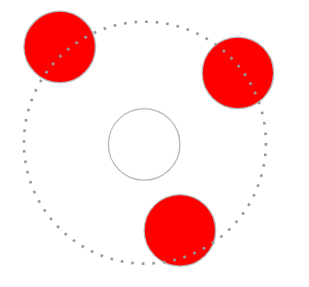
\includegraphics[width=\linewidth]{diagrams/visual_field.PNG}
            \caption{Visual field of an agent.}
            \label{fig:3.1a}
        \end{subfigure}
        \begin{subfigure}[b]{0.3\linewidth}
            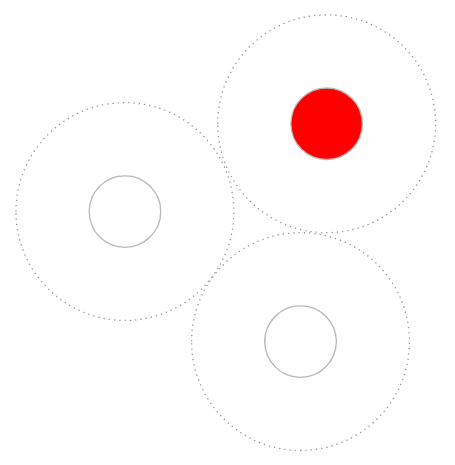
\includegraphics[width=\linewidth]{diagrams/social_distancing.PNG}
            \caption{Social Distancing: The three agents here, two healthy and one diseased, show their social distance boundary.}
            \label{fig:3.1b}
        \end{subfigure}
        \caption{}
    \end{figure}

    \subsection{Deflections}\label{subsec:deflections}
    The social distancing approach discussed above is too strict and not flexible to simulate realistic social-distancing.
    So, we introduced a concept called deflections that enable more flexible social distancing behaviours.
    When an agent sees a neighbour, it can take an action of moving towards it, or an action of moving away from it.
    We termed these actions as deflections.
    Deflections are rules specific to each agent which dictate whether to move towards or away from another agent in its vicinity and how strongly.
    A repulsive force is represented as a negative scalar while the attractive force is represented as a positive scalar.

    An agent can act differently based on the state of its neighbour.
    For example, the agent would like to move towards a healthy agent and away from a diseased agent.
    Likewise, the agent can have different behaviour based on its own state.
    For example, a diseased agent might want to move away from a recovered neighbour and get attracted towards another diseased agent.
    Finally, we end up with a force value for each pair of states except the dead state i.e.
    \{(healthy, diseased), (healthy, recovered), \ldots \}, a total of 9 scalar values.
    They are represented in a 3x3 matrix where each row represents the state of the agent and each column representing states of its neighbour.
    We can see these deflection matrix in the figure\ref{fig:4.2}.
    When there are more than one neighbour in the visual field, then the deflection force vectors from all the neighbours are summed and normalized for the final deflection force.

    One can imagine how perfect deflections for an agent might look like.
    We defined perfect deflections as attraction on the pairs: \{(healthy, healthy), (healthy, recovered), (recovered, recovered), (diseased, diseased)\} and repulsion on pairs: \{(healthy, diseased), (recovered, diseased)\}.
    This deflection matrix can be seen in figure\ref{fig:4.2c}.
    This ensures that no healthy or recovered agent tries to stick around with a diseased agent, thus, reducing the spread of the disease.

    \subsection{Herd Immunity}\label{subsec:herd-immunity}
    We modeled herd immunity\cite{herdImm} by changing the deflection of (recovered, recovered) to repulsion in the perfect deflections.
    With this, the recovered agents try to spread around in the environment.
    Because recovered agents cannot get diseased directly, it lowers the overall probability of disease percolation.

    The type of deflections and their effects on the percolation is not limited to the experiments we have conducted, there may be more interesting permutations of deflections.
    One more interesting permutation includes perfect deflections with repulsion between healthy agents.
    This shows a social distancing phenomenon not only between different groups but also between the individuals of the same group.

    \subsection{Evolution}\label{subsec:evolution}
    One major question we asked ourselves is "Can we evolve deflections?".
    We then made an attempt to test the hypothesis.
    We ran the simulation for 400 episodes where each episode is 1500 time-steps.

    \subsubsection{Genes}
    We considered the deflection matrix as the genes of the agents.
    The genes remain unchanged throughout the agent's lifetime.
    The system starts out with random deflections.

    \subsubsection{Performance Metric}
    After each episode, the agents' score is calculated from the formula below:

    \begin{equation}
        score = \frac{nEpisodes}{nDiseased + nSpread}
    \end{equation}
    Here $nEpisodes$ is the number of episodes the agent survived.
    $nDiseased$ is the number of times the agent got diseased.
    And $nSpread$ is the number of neighbours the agent spread its disease to.

    This formula penalizes the score of the agents that get diseased often or that spreads the disease often.
    It rewards the agents which survive the episode.
    This way, we can drive the evolution to maximize survival and minimize death.

    \subsubsection{Selection Mechanism}
    After each episode, we select the agents for next episode with the following criteria:

    \begin{itemize}
        \item 50\% of the agents of the next episode are taken directly from the best half of the previous episode.
        \item 40\% of the agents are mutated copies of the agents of the previous episode picked with a probability proportional to its score.
        This is also called roulette wheel probability.
        The mutation is performed by adding a small random value between in the range [-0.1, 0.1] to the deflections element-wise.
        \item 10\% of the agents are new agents with random deflections.
    \end{itemize}

    The idea behind this approach is that as agents with genes that try to attract towards diseased agents will tend to get infected, this will result in a low score.
    But the agents that repel diseased agents will have lower probability of getting infected, scoring higher.
    In this way, the system will eventually leave out the agents with bad genes and propagate the fitter genes through the episodes.
    In practice, however, this kind of evolution is not monotonic.
    The following section contains further details on this.

    \section{Results}\label{sec:results}
    We ran the simulation and took observations for many parameter combinations.
    Due to a large number of possibilities in varying the parameters, we filtered out the most interesting combinations and assigned serial numbers (SN\{1, 2, \ldots \}) to them.
    We ran the simulation for 1500 time-steps.
    They are as follows:

    \begin{itemize}

        \item Base model
        \begin{itemize}
            \item[SN1:] Vanilla base model
            \item[SN2:] High death rate
            \item[SN3:] High recovery rate
            \item[SN4:] Low recovery rate
            \item[SN5:] High contagion rate
            \item[SN6:] High recovery loss rate
            \item[SN7:] Social distancing
        \end{itemize}

        \item Perfect deflections model
        \begin{itemize}
            \item[SN8:] Vanilla perfect deflections
            \item[SN9:] No overlap between the agents
            \item[SN10:] Social distancing
            \item[SN11:] Social distancing after 20\% of the population gets diseased
            \item[SN12:] Social distancing disabled for like-agents (with same state)
            \item[SN13:] 3x increase in deflection force
            \item[SN16:] Repulsion between recovered agents
        \end{itemize}

        \item Evolutionary model
        \begin{itemize}
            \item[SN14:] Beginning of the evolution
            \item[SN15:] End of the evolution
        \end{itemize}

    \end{itemize}

    \begin{figure}[ht]
        \centering
        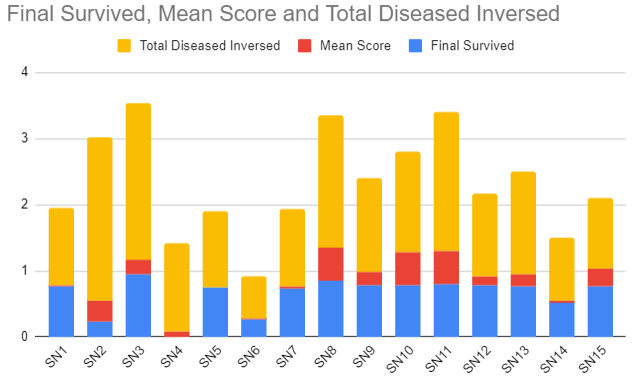
\includegraphics[width=0.5\linewidth]{diagrams/All_SNs.png}
        \caption{Performance of all cases}
        \label{fig:4.1}
    \end{figure}

    \textbf{SN1:} The base vanilla model is tuned to match the standard SIR model as seen in figure\ref{fig:SN1}.
    We will be comparing other cases with this base model to make judgements.
    \textbf{SN2:} From the figures\ref{fig:4.1} and\ref{fig:SN2}, we see that when death rate of a disease is high, then the disease doesn't spread as much.
    This is good for the goal of this project, but many agents die in the process.
    \textbf{SN3:} A better outcome is seen in the next case where we increased the recovery rate to a high value.
    As in figure\ref{fig:SN3} the spread is small because as agents get infected, the soon recover and do not further spread the disease.
    \textbf{SN4:} We then lowered the recovery rate and the outcome was disastrous as seen in figure\ref{fig:SN4}.
    \textbf{SN5:} Having high contagion rate is not as bad as having low recovery rate, this is seen in the figures\ref{fig:4.1} and figure\ref{fig:SN5}.
    \textbf{SN6:} However, the worst case of all turned out to be the one where the recovered agents lose their immunity quickly.
    As seen in figure\ref{fig:SN6}, the number of diseased agents does not drop throughout the run.
    \textbf{SN7:} When we enabled length based social distancing\cite{3b1b}, the system took longer to reach outbreak (the point in the population graph where number of diseased is equal to the number of healthy) as seen in figure\ref{fig:SN7}.
    Although social distancing helped prolong the spread of the disease, the system still had an outbreak.
    Increasing the social distance made the outbreak happen later in time.

    \begin{figure}[H]
        \centering
        \begin{subfigure}[b]{0.49\linewidth}
            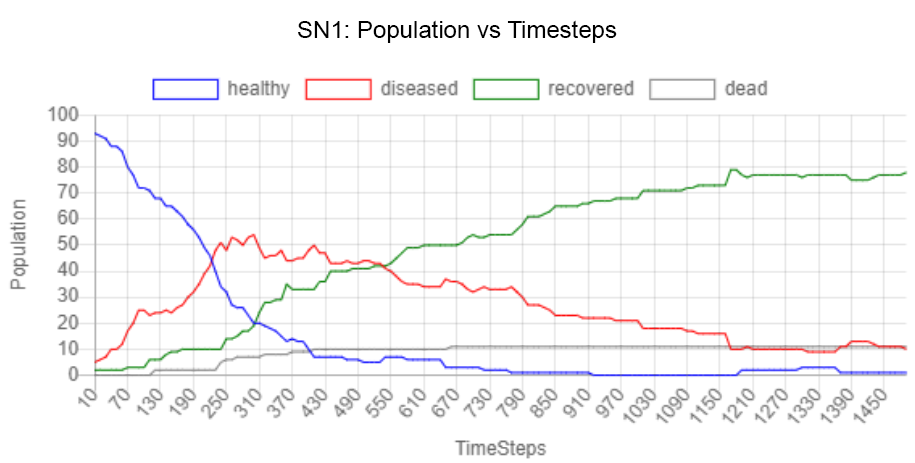
\includegraphics[width=\linewidth]{pop_graphs/SN1_pop.png}
            \caption{SN1: Vanilla base model}
            \label{fig:SN1}
        \end{subfigure}
        \begin{subfigure}[b]{0.49\linewidth}
            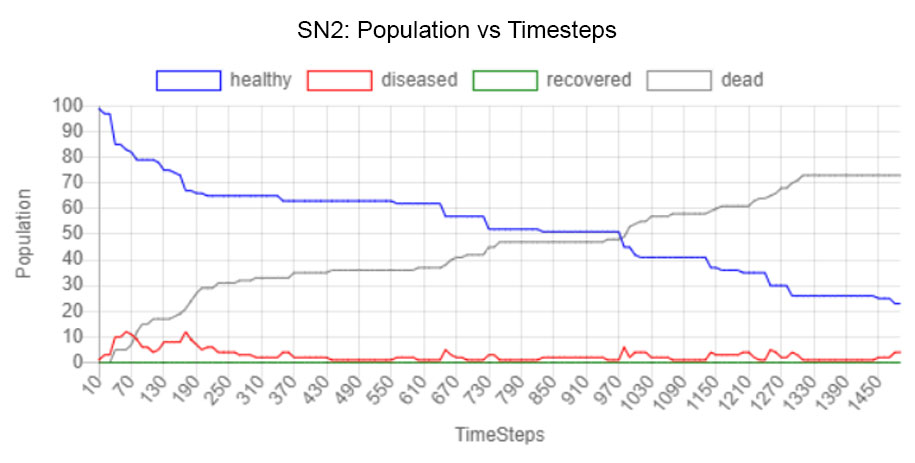
\includegraphics[width=\linewidth]{pop_graphs/SN2_pop.png}
            \caption{SN2: High death rate}
            \label{fig:SN2}
        \end{subfigure}
        \begin{subfigure}[b]{0.49\linewidth}
            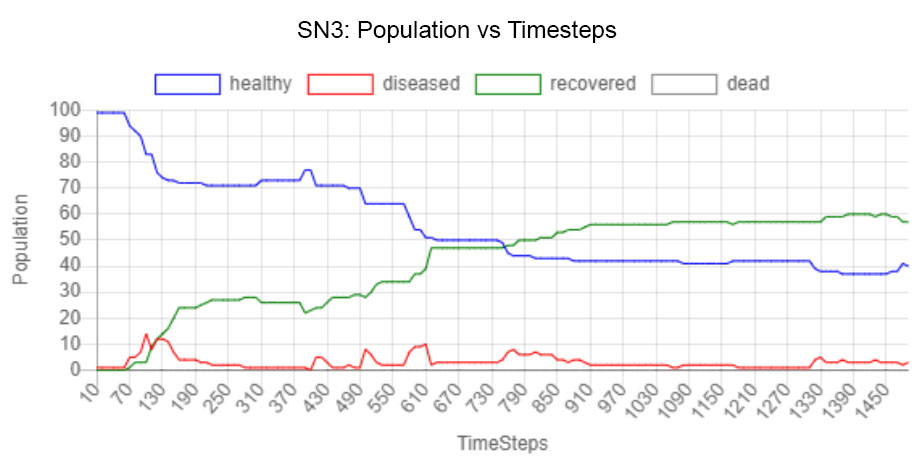
\includegraphics[width=\linewidth]{pop_graphs/SN3_pop.jpg}
            \caption{SN3: High recovery rate}
            \label{fig:SN3}
        \end{subfigure}
        \begin{subfigure}[b]{0.49\linewidth}
            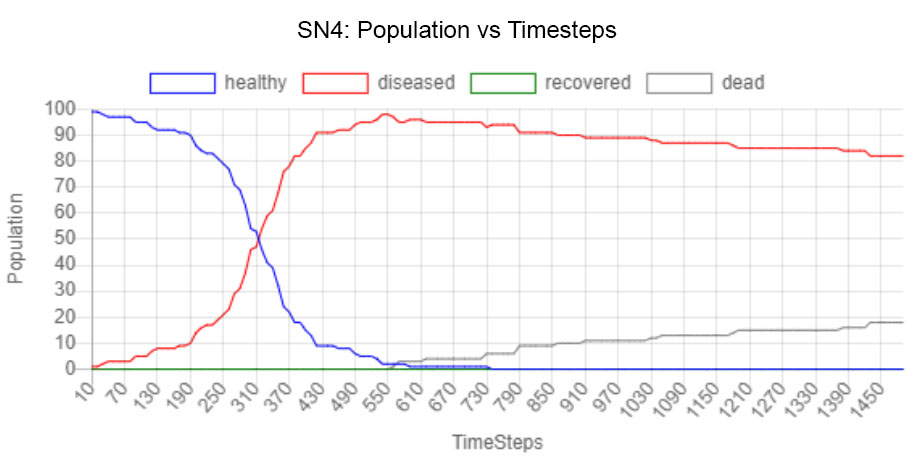
\includegraphics[width=\linewidth]{pop_graphs/SN4_pop.jpg}
            \caption{SN4: Low recovery rate}
            \label{fig:SN4}
        \end{subfigure}
        \begin{subfigure}[b]{0.49\linewidth}
            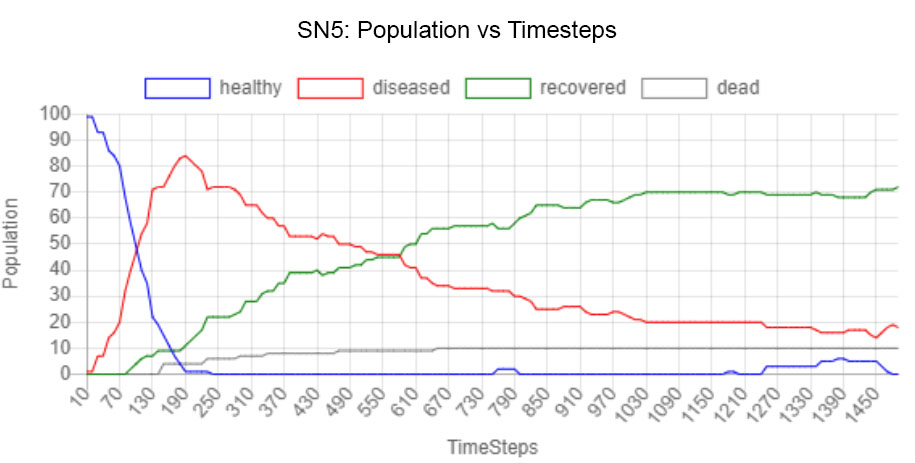
\includegraphics[width=\linewidth]{pop_graphs/SN5_pop.jpg}
            \caption{SN5: High contagion rate}
            \label{fig:SN5}
        \end{subfigure}
        \begin{subfigure}[b]{0.49\linewidth}
            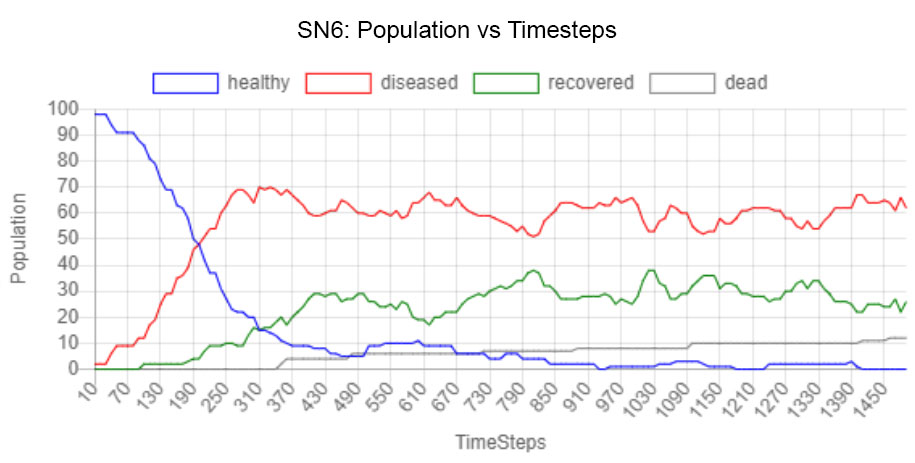
\includegraphics[width=\linewidth]{pop_graphs/SN6_pop.jpg}
            \caption{SN6: High recovery loss rate}
            \label{fig:SN6}
        \end{subfigure}
        \begin{subfigure}[b]{0.49\linewidth}
            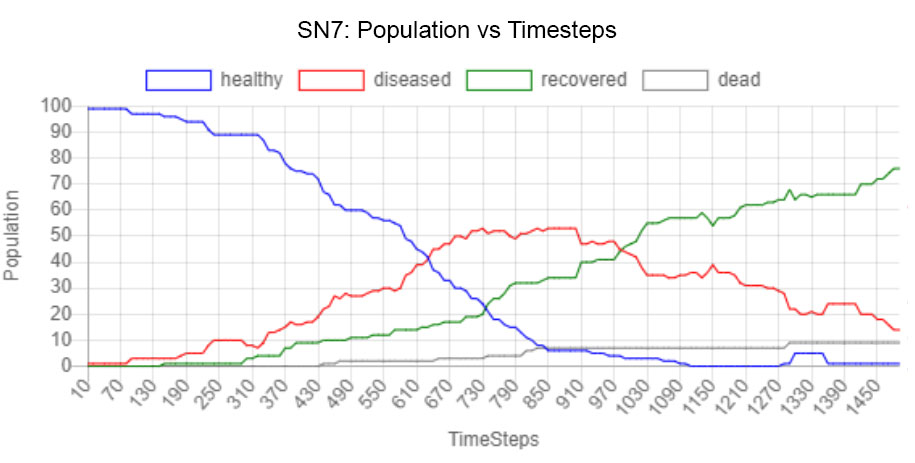
\includegraphics[width=\linewidth]{pop_graphs/SN7_pop.jpg}
            \caption{SN7: Social distancing}
            \label{fig:SN7}
        \end{subfigure}
        \caption{Population graphs of base model variants}
    \end{figure}

    \textbf{SN8:} When we introduced perfect deflections into the system, many interesting patterns emerged.
    All the healthy and recovered agents form small groups from randomness.
    They resist coming close to diseased agents, which form their own groups.
    Formation of these groups is analogous to forming social gatherings between healthy agents and restraining diseased agents into quarantine cells.
    Ideally, this type of behaviour will restrict the spread of the disease completely and that is what we see in some simulations shown in figure\ref{fig:SN8T1}.
    However, there is one major flaw in this system.
    Whenever an agent inside a group of healthy ones gets infected, then almost all the agents in that group get infected.
    The diseased population suddenly bursts into a large number.
    We see this in figure\ref{fig:SN8T3}.
    Sometimes, this system spreads the disease and follows a similar trend to the base model, this is seen in figure\ref{fig:SN8T2}.

    We then modified this model with a few variations.
    \textbf{SN9:} We removed the overlapping rule and made the agents collide with each other.
    We observed a pattern that is very similar to swarm or flock where a large group of agents move in sync and form a macro-organism.
    However, due to this change, the gap between two agents becomes smaller on the whole and the probability of being in the vicinity of a diseased agent rises.
    \textbf{SN10:} We also added length based social distancing among all agents which had a similar effect to the previous case.
    \textbf{SN11:} We then enabled social distancing after 20\% of the population gets diseased\cite{3b1b}.
    This is better than the base model, but suffers the problems of SN9.
    \textbf{SN12:} Now, we enabled overlapping and added length based social distancing to agents of different state.
    This produced the most robust model we have seen in our experiments as seen in the figure\ref{fig:4.1}.
    In half of the cases, the disease does not even cause an outbreak, similar to the figure\ref{fig:SN8T1}.
    \textbf{SN13:} Since the perfect deflection model is so good, we tried increasing the strength of the deflections by 3.
    The agents immediately become flock-like and form dense groups.
    The disease-burst problem gets worse in this scenario and majority of the population gets diseased at once.

    \begin{figure}[H]
        \centering
        \begin{subfigure}[b]{0.49\linewidth}
            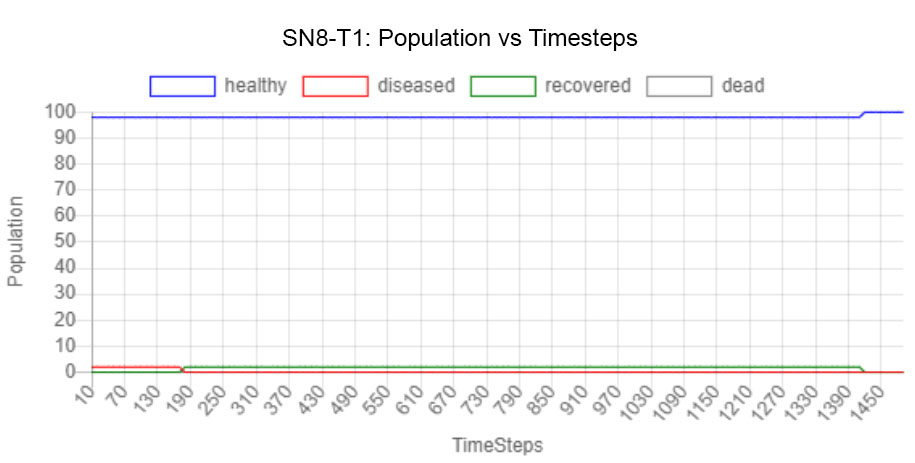
\includegraphics[width=\linewidth]{pop_graphs/SN8-T1_pop.jpg}
            \caption{SN8: Vanilla perfect deflections, type 1}
            \label{fig:SN8T1}
        \end{subfigure}
        \begin{subfigure}[b]{0.49\linewidth}
            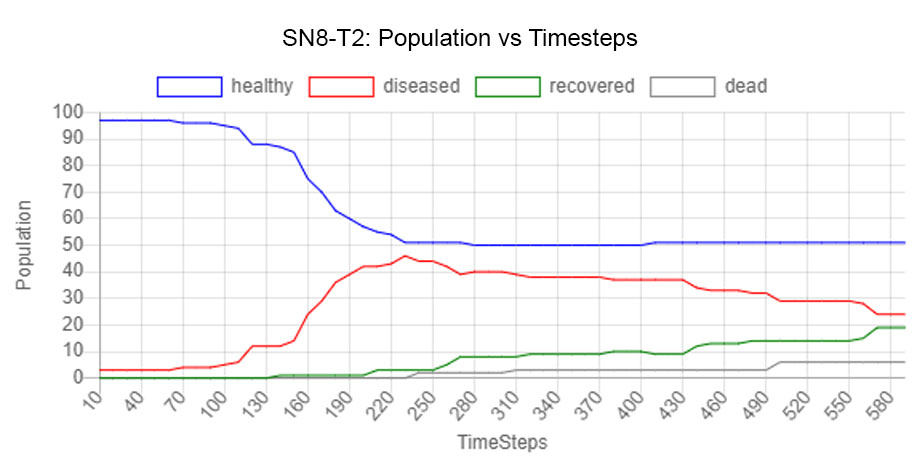
\includegraphics[width=\linewidth]{pop_graphs/SN8-T2_pop.jpg}
            \caption{SN8: Vanilla perfect deflections, type 2}
            \label{fig:SN8T2}
        \end{subfigure}
        \begin{subfigure}[b]{0.49\linewidth}
            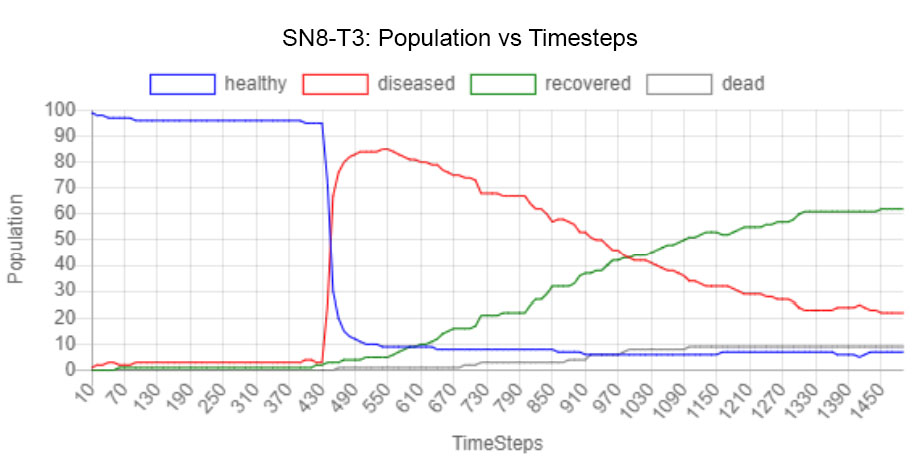
\includegraphics[width=\linewidth]{pop_graphs/SN8-T3_pop.jpg}
            \caption{SN8: Vanilla perfect deflections, type 3}
            \label{fig:SN8T3}
        \end{subfigure}
        \begin{subfigure}[b]{0.49\linewidth}
            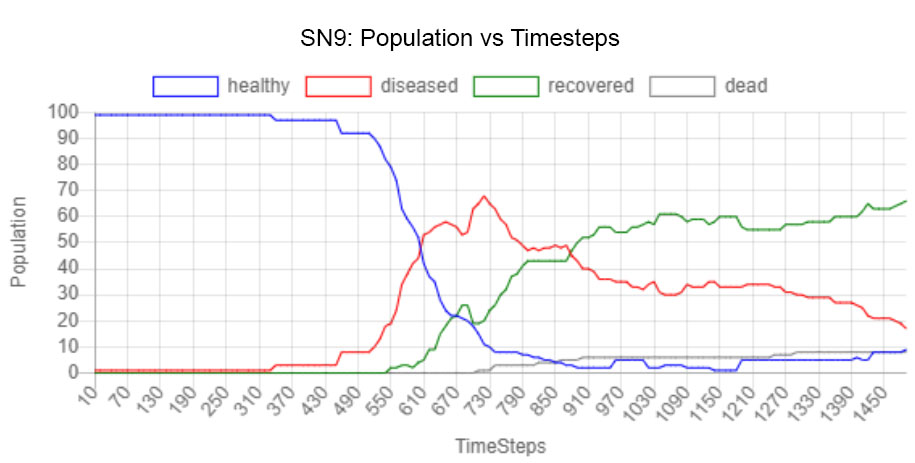
\includegraphics[width=\linewidth]{pop_graphs/SN9_pop.jpg}
            \caption{SN9: No overlap between the agents}
            \label{fig:SN9}
        \end{subfigure}
        \begin{subfigure}[b]{0.49\linewidth}
            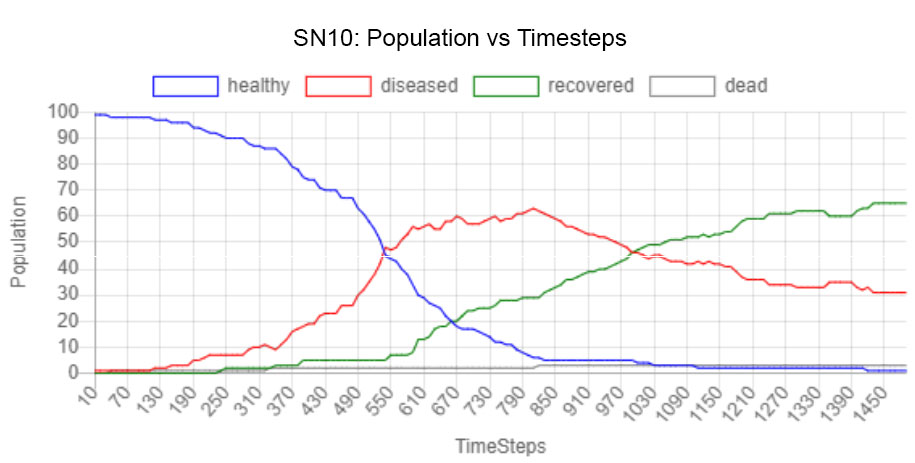
\includegraphics[width=\linewidth]{pop_graphs/SN10_pop.jpg}
            \caption{SN10: Social distancing on perfect deflections}
            \label{fig:SN10}
        \end{subfigure}
        \begin{subfigure}[b]{0.49\linewidth}
            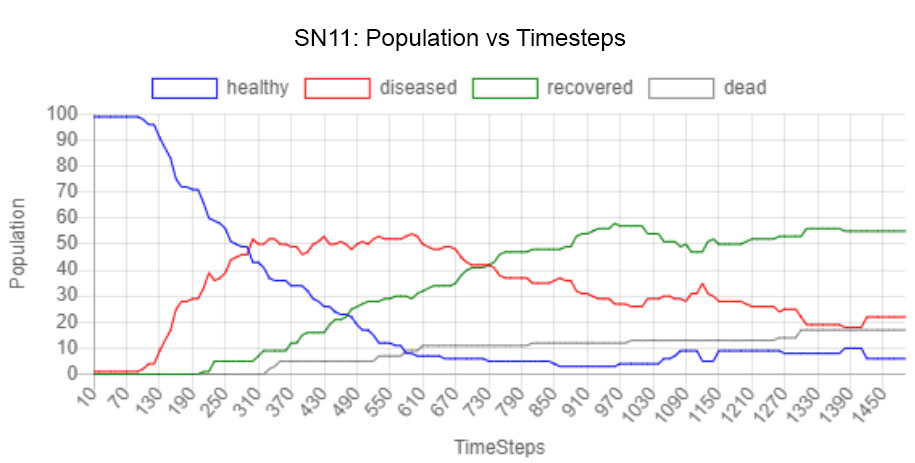
\includegraphics[width=\linewidth]{pop_graphs/SN11_pop.jpg}
            \caption{SN11: Social distancing after 20\%}
            \label{fig:SN11}
        \end{subfigure}
        \caption{Population graphs of deflection model variants}
    \end{figure}

    \textbf{SN14  \& SN15:} Finally, we ran the evolutionary algorithm and the results were quite outstanding.
    The evolution started off with random genes as shown in figure\ref{fig:4.2a}.
    The population graph at the beginning of the evolution is seen in figure\ref{fig:SN14} which is similar to the base model as expected.
    After 400 episodes, the model evolved genes shown in figure\ref{fig:4.2b} that are somewhat similar to the perfect deflections defined as figure\ref{fig:4.2c}.
    We also see in Figure\ref{fig:4.1} that the evolved model performs better than the same model at the beginning of the evolution and is slightly better than the base model, but much weaker than the model of perfect deflection (SN8).
    The model learned to maintain social distancing in order to prevent the disease.
    This shows that the evolutionary algorithm works.
    The population graph of the evolved model is similar to that of SN8, the system with perfect deflections.
    The mean score of all the agents in the system keeps increasing overtime as seen in the figure\ref{fig:4.3} due to the selection process.

    One striking difference that we see in the evolved genes is that the deflection between the recovered agents is repulsive.
    This is exactly what we did to achieve herd immunity.
    It was surprising to see the evolution figure that out.

    \begin{figure}[h]
        \centering
        \begin{subfigure}[b]{0.32\linewidth}
            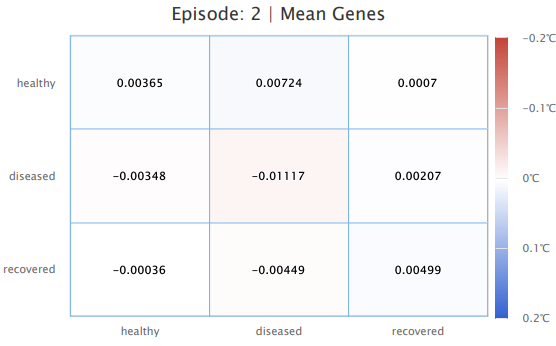
\includegraphics[width=\linewidth]{diagrams/SN14_MeanGenes.PNG}
            \caption{Mean genes before evolution}
            \label{fig:4.2a}
        \end{subfigure}
        \begin{subfigure}[b]{0.33\linewidth}
            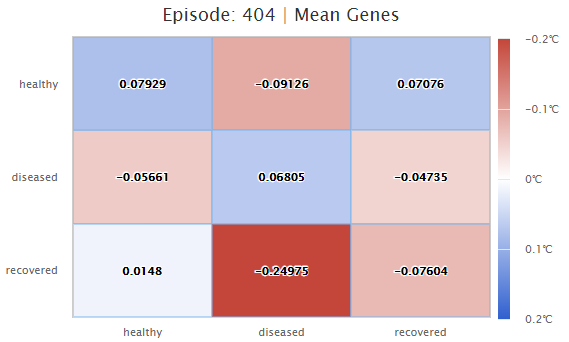
\includegraphics[width=\linewidth]{diagrams/SN15_MeanGenes.PNG}
            \caption{Mean genes after evolution}
            \label{fig:4.2b}
        \end{subfigure}
        \begin{subfigure}[b]{0.33\linewidth}
            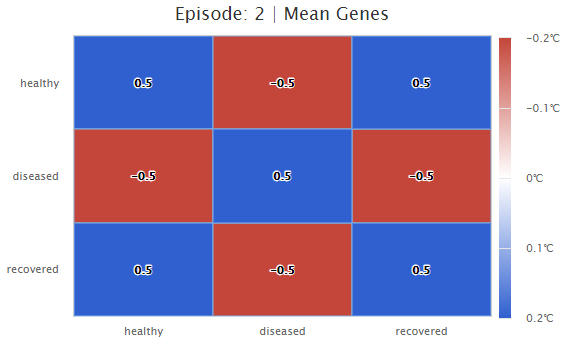
\includegraphics[width=\linewidth]{diagrams/perfect_genes.PNG}
            \caption{Perfect deflections}
            \label{fig:4.2c}
        \end{subfigure}
        \caption{Mean Genes}
        \label{fig:4.2}
    \end{figure}

    \begin{figure}[ht]
        \centering
        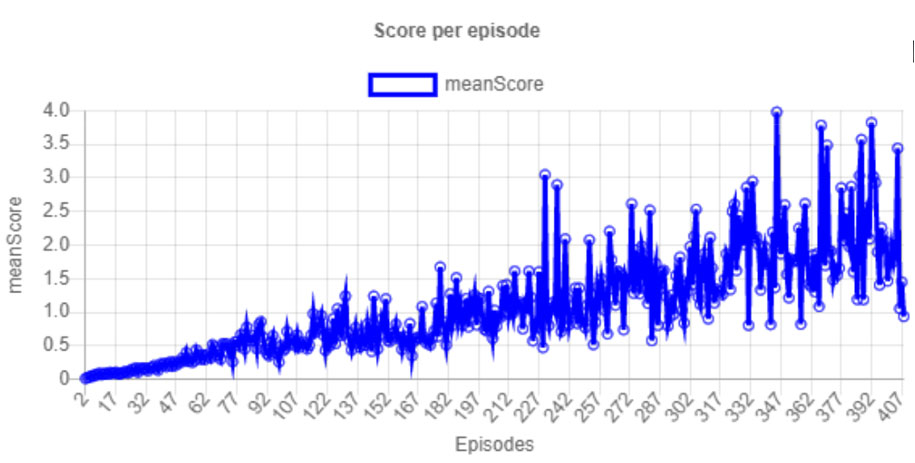
\includegraphics[width=0.5\linewidth]{diagrams/score_plot.jpg}
        \caption{Scores for each episode in the evolution}
        \label{fig:4.3}
    \end{figure}

    \begin{figure}[H]
        \centering
        \begin{subfigure}[b]{0.49\linewidth}
            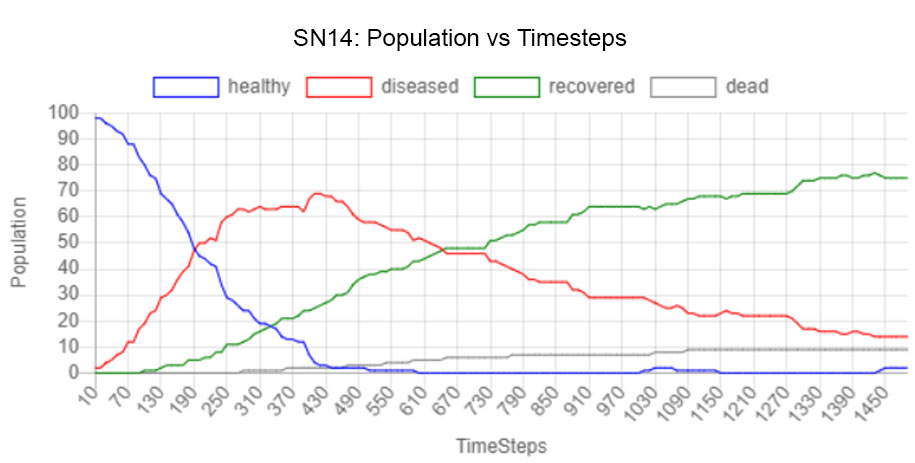
\includegraphics[width=\linewidth]{pop_graphs/SN14_pop.jpg}
            \caption{SN14: Beginning of the evolution}
            \label{fig:SN14}
        \end{subfigure}
        \begin{subfigure}[b]{0.49\linewidth}
            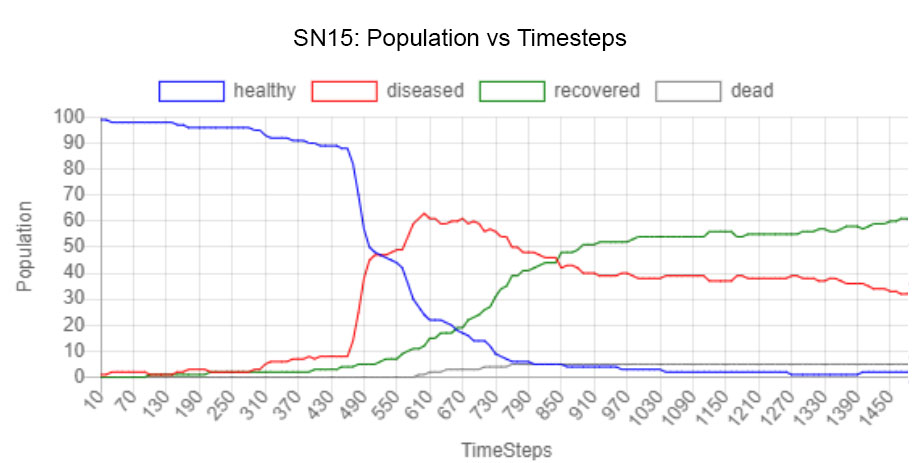
\includegraphics[width=\linewidth]{pop_graphs/SN15_pop.jpg}
            \caption{SN15: End of the evolution}
            \label{fig:SN15}
        \end{subfigure}
        \caption{Population graphs of evolutionary model.}
    \end{figure}

    \section{Conclusion}\label{sec:conclusion}
    We have successfully demonstrated that social distancing is a key factor in preventing the percolation of a disease in a highly active and dynamic system.
    We also demonstrated that herd immunity helps in this process.
    Furthermore, we evolved the system itself to mitigate the spread and it resulted in a system with social distancing and herd immunity.
    One issue with the evolutionary process we found is that it follows preferential attachment\cite{barabasi} where the agents of the higher score will always remain in the system even if they have a few bad deflections in their genes.
    Another issue is that the evolved system will always have agents with random deflections due to the selection process.
    These limitations will never let evolution reach 100\% perfection.

    \printbibliography

\end{document}